\documentclass[12pt,a4paper]{cibb}

\usepackage{subfigure,graphicx}
\usepackage{amsmath,amsfonts,latexsym,amssymb,euscript,xr}
\usepackage{multirow}
\usepackage{hyperref}
\usepackage{svg}

\title{\large $\ $\\ \bf ON SECONDARY STRUCTURE ANALYSIS BY USING FORMAL GRAMMARS AND ARTIFICIAL NEURAL NETWORKS}

\author{ Polina Lunina$^{(1,2)}$, Semyon Grigorev$^{(1,2)}$}
\address{$\ $\\(1) Saint Petersburg State University, 7/9 Universitetskaya nab., St. Petersburg, 199034, Russia\\
 lunina\_polina@mail.ru, s.v.grigoriev@spbu.ru
\\
%
\bigskip
(2) JetBrains Research, Primorskiy prospekt 68-70, Building 1, St. Petersburg 197374, Russia\\
semyon.grigorev@jetbrains.com
}



\abstract{DNN, CNN, Machine Learning, Secondary Structure, Genomic Sequences, Formal Grammars, Parsing.
\\[17pt]
{\bf Abstract.}
A way to combine formal grammars and artificial neural networks for biological sequences processing was recently proposed.
In this approach, an ordinary grammar encodes primitive features of the secondary structure of RNA, parsing is utilized for features extraction and artificial neural network~--- for processing of the extracted features.
Parsing is a bottleneck of the approach: input sequences should first be parsed before processing with a trained model which is a time-consuming operation when working with huge biological databases.
In this work we solve the problem by employing staged learning and limiting parsing to be used only during network training.
We also compare networks which represent the parsing result in two different ways: by a vector and a bitmap image.
Finally, we evaluate our solution on tRNA classification.}

\begin{document}
\thispagestyle{myheadings}
\pagestyle{myheadings}
\markright{\tt Proceedings of CIBB 2019}%check year



\section{\bf Introduction}

Development of effective computational methods for genomic sequences analysis is an open problem in bioinformatics.
While the existing algorithms for sequences classification and subsequences detection adopt different concepts and approaches, they share one idea: secondary structure of genomic sequences contains important information about biological functions of organisms.
There are different ways to handle secondary structure, for example, probabilistic grammars and covariance models~\cite{EddyDurbin, dowell2004evaluation, knudsen1999rna}.

Real-world biological data commonly contains different mutations, noise, and random variations.
This issue requires some sort of probability estimation while modeling the secondary structure.
Probabilistic grammars and covariance models provide such functionality, are expressive and handle long-distance connections.
They are successfully used in practical tools, such as Infernal~\cite{Infernal}, but building and training accurate grammar or model for predicting the whole secondary structure involves theoretical and practical difficulties.
On the other hand, artificial neural networks are a common way to process noisy data and find complex structural patterns.
Moreover, the efficiency of neural networks for genetic data processing has already been shown in some works~\cite{Humidor,ANN}.

An approach for biological sequences processing which employs the combination of ordinary formal grammars and artificial neural networks was proposed in~\cite{grigorevcomposition}.
The key idea is to use an ordinary context-free grammar to describe only basic secondary structure features and leave the probabilistic analysis to the neural network which takes parsing-provided data as an input.

Secondary structure of RNA sequences can be viewed as a composition of stems~\cite{MQbioinformatics19}.
Grammar $G_0$ provided in~\cite{grigorevcomposition} considers only the conventional base pairs and describes the recursive composition of stems which are at least three base pairs in height, and we use this grammar in our paper.
The result of a parsing algorithm for the input string $w$ and the fixed grammar non-terminal $N$ (start nonterminal) is an upper-triangular boolean matrix $M_N$, where $M_N [i,j] = 1$, iff the substring $w[i,j-1]$ is derivable from $N$.
This means that, for the grammar $G_0$, a matrix contains $1$ in a cell iff a correspondent substring folds to a  stem of height at least 3.
A stem results in a diagonal chain of $1$ in the matrix, if its height is more than 3.
Figure~\ref{fig:example} presents the parsing result of a sequence

\[
w_1 = CCCCATTGCCAAGGACCCCACCTTGGCAATCCC
\]

w.r.t the grammar $G_0$.
Colored boxes map a substring which folds to a stem to correspondent cells in the matrix.

\begin{figure}[h]
\begin{center}
\centering
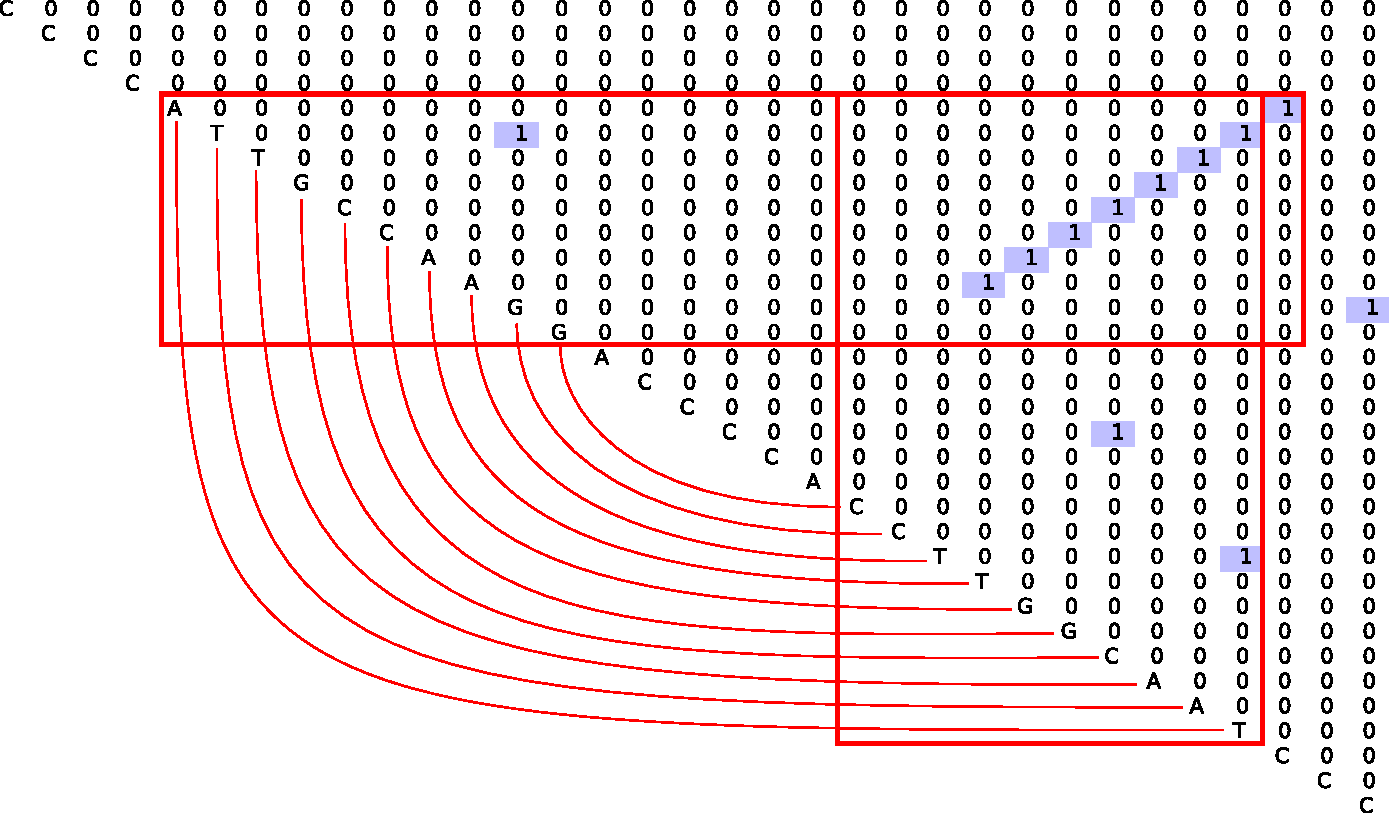
\includegraphics[width=0.8\textwidth]{figures/4.pdf}
\caption{Parsing result for sequence which should fold to
stem}
\label{fig:example}
\end{center}
\end{figure}

The parsing result in a form of matrix can be linearized, compressed into a byte or int vector, and be further handled by a dense neural network, as described in~\cite{grigorevcomposition}.
Unfortunately, linearization breaks data locality: a chain of $1$, which signifies a high stem, is local in a matrix, but is broken apart during its linearization.
We see it to be an argument to investigate the applicability of convolutional networks for parsing result handling as a boolean matrix can be converted to a black-white bitmap image.
In this paper we provide an empirical comparison of networks which handle vectors and images.

Another problem is a bad performance of the earlier solution.
Since the trained network handles parsing result, each input sequence should first be parsed.
Parsing is a very time-consuming step: context-free parsing has cubic complexity in terms of the input length.
Even if we use matrix-based parsing algorithm~\cite{Azimov:2018:CPQ:3210259.3210264} which utilizes GPGPU, performance is insufficient.
We believe it would be better to avoid the parsing step.
In this work, we propose a solution to this problem by building a network which handles raw sequences, not parsing results.

\section{\bf The solution}

In this paper we improve the solution proposed in~\cite{grigorevcomposition}.
First, we describe how to use convolutional network for parsing result processing.

Parsing result is a boolean matrix and we utilize the artificial neural network to detect sufficient features and to find patterns in their appearance.
Therefore, we need to transform these boolean matrices to a data structure accepted by the neural network.
Presently, we came up with two possible ways.

The first one is to drop out the nullary bottom left triangle, vectorize the top right triangle row by row and transform it into a byte vector.
This approach reduces the input size, but it requires all the input sequences to have equal length.
Thus we propose to either cut sequences to be of some predefined length or to pad them up with some blank symbols.
Vectorisation breaks data locality which makes learning harder: the network should restore back the relations broken during linearization.
This also means that the learning takes more time.

The second way is to represent the matrix as an image: the false bits of the matrix as white pixels and the true bits as black ones.
This approach makes it possible to process sequences of different lengths since the images are easily transformed to a specified size.
Data locality is also preserved: the information about relative positions of extracted basic features does not get lost which should improve learning.

To handle images, we use a network which consists of a small number of convolutional layers, linearization, and dense network which has a similar architecture as for vectorized data.
The example of such network is presented in figure~\ref{nn}, block \textbf{\texttt{N1}}.
In this paper we provide an evaluation on both data formats and compare the results.

To create a network which can handle original sequence instead of its parsing matrix, we propose to use two-staged learning.
In this approach, a network is built in two stages: first, a network is trained which solves a subtask and then it is used as pretrained layers in the training of the resulting network.
In our solution we first train a neural network to handle parsing results which performs classification according to a problem at hands.
We create two networks in order to compare different architectures: one of them handles vectorized parsing result, the other handles parsing result represented as a bitmap image.
After that, we extend this neural network by a number of input layers that take the initial nucleotide sequence as an input and convert it to the parsing result which is handled appropriately by the pretrained layers.

A figure~\ref{nn} presents a detailed description of the three neural networks.
Here \textbf{\texttt{N1}} is a network which handles images, \textbf{\texttt{N2}} is a network which handles vectorized parsing results, and \textbf{\texttt{N0}} is an additional block which converts the input sequence into a set of features which can be handled by using \textbf{\texttt{N1}} or \textbf{\texttt{N2}}.

To sum up, we built a network that handles sequences and requires parsing only for training the network it is based on.
This removes the parsing step from the usage of the trained model.


\section{\bf Experiments}

We evaluate the proposed approach with the described above modifications on two tRNA sequences analysis tasks.
The first one is a classification of tRNA into two classes: eukaryotes and prokaryotes, while the second is a classification into four classes: archaea, bacteria, plants and fungi.
We use sequences from tRNA databases~\cite{trnadb1,trnadb2} for these experiments.
We select the equal number of samples (single tRNA molecule sequences) for each class for both classification tasks.
Each sample was parsed w.r.t. the grammar $G_0$ from the earlier paper and then both vectorized and transformed into an image.
After that, we trained two neural networks: one which handles the representation of the parsing result as vectors, and the second~--- as images.
Finally, we train the extended neural network.
It consists of a block which takes an initial tRNA sequence as an input and transforms it into the parsing result by few dense layers with batch normalization and the block of pretrained layers: either the vector- or the image-based models from the previous step.

These neural networks for two classes classification are shown in the figure~\ref{nn}, where \textbf{\texttt{N2}} represents the model that handles vectors, \textbf{\texttt{N1}} represents the network which classifies images and \textbf{\texttt{N0}} is the extension that transforms a sequence to the parsing result.
For vector-based network, we combine this extension and the whole original sequence of layers.
For image-based network, we use the similar architecture, except we remove the convolutional layer from the extended model, thus, the first layer at the junction of the blocks corresponds to the linearized image.

\begin{figure}[h]
\begin{center}
\centering
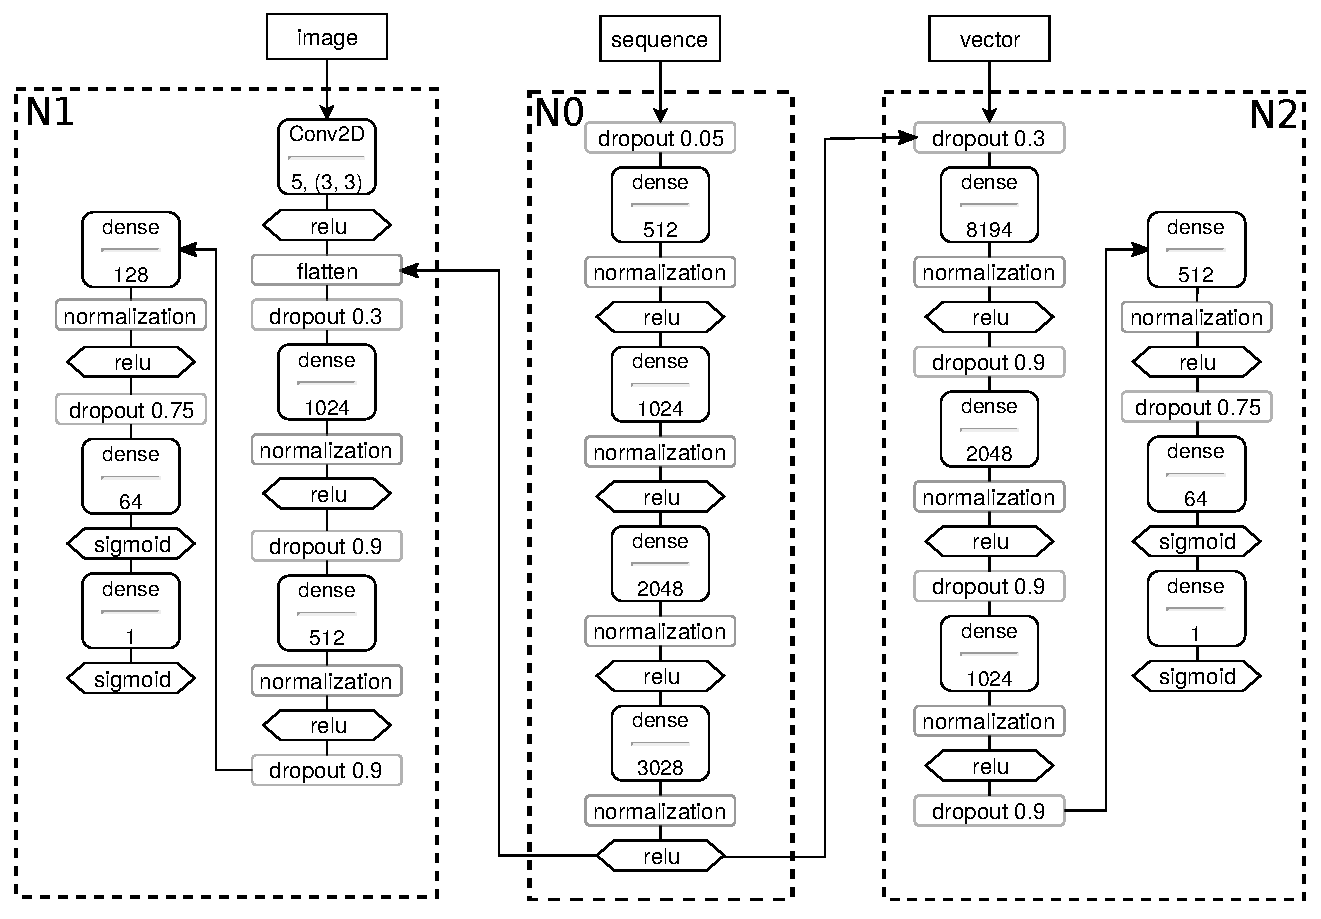
\includegraphics[width=14cm]{nn_arch.pdf}
\caption{Neural networks architectures}
\label{nn}
\end{center}
\end{figure}


All extended neural networks were trained, validated (by hold-out validation) and tested on the same datasets as the corresponding base ones.
The trained models for two classes (EP) and for four classes (ABFP) classification tasks were estimated by using classical machine learning metrics: accuracy, precision and recall.

Accuracy metrics for each problem for the test datasets are presented in the table~\ref{acc}, where base model is a model which handles parsing result (image or vector respectively) and extended model handles tRNA sequences and extends the corresponding base model.

\begin{table}[h]
\centering
\caption{Base and extended models test results by accuracy metrics}
\begin{tabular}{|l||l|l||l|l|}
\hline
Classifier                                                               & \multicolumn{2}{l||}{EP}               & \multicolumn{2}{l|}{ABFP}           \\ \hline \hline
Approach                                                                 & Vector-based       & Image-based      & Vector-based      & Image-based     \\ \hline
\begin{tabular}[c]{@{}l@{}}Base model\\ accuracy\end{tabular}            & 94.1\%             & 96.2\%           & 86.7\%            & 93.3\%          \\ \hline
\begin{tabular}[c]{@{}l@{}}Extended model \\ accuracy\end{tabular}       & 97.5\%             & 97.8\%           & 96.2\%            & 95.7\%          \\ \hline
\begin{tabular}[c]{@{}l@{}}Total training \\ time\end{tabular}       & 30000s             & 4600s           & 31800s            & 3600s          \\ \hline
\begin{tabular}[c]{@{}l@{}}Samples for\\ train:valid:test\end{tabular} & \multicolumn{2}{l||}{\begin{tabular}[c]{@{}l@{}}20000:5000:10000\\ (57\%:14\%:29\%)\end{tabular}} & \multicolumn{2}{l|}{\begin{tabular}[c]{@{}l@{}}8000:1000:3000\\ (67\%:8\%:25\%)\end{tabular}} \\ \hline
\end{tabular}
\label{acc}
\end{table}


The estimations of precision and recall metrics for extended models for both classifiers on the same  samples as in table~\ref{acc} are presented in the table~\ref{pe}.

\begin{table}[h]
\centering
\caption{Models test results by precision and recall metrics for each class}
\begin{tabular}{|l||l|l|l|l|l|}
\hline
\multirow{2}{*}{Classifier} & \multirow{2}{*}{Class} & \multicolumn{2}{l|}{Vector-based approach} & \multicolumn{2}{l|}{Image-based approach} \\ \cline{3-6} 
                            &                        & precision         & recall        & precision        & recall        \\ \hline \hline
\multirow{2}{*}{EP}         & prokaryotic            & 95.8\%            & 99.4\%        & 96.2\%           & 99.4\%        \\ \cline{2-6} 
                            & eukaryotic             & 99.4\%            & 95.6\%        & 99.4\%           & 99.5\%        \\ \hline \hline
\multirow{4}{*}{ABFP}       & archaeal               & 91.1\%            & 99.2\%        & 91.6\%           & 98.5\%        \\ \cline{2-6} 
                            & bacterial              & 96.6\%            & 95.1\%        & 95.2\%           & 95.5\%        \\ \cline{2-6} 
                            & fungi                  & 98.5\%            & 94.9\%        & 97.5\%           & 94.3\%        \\ \cline{2-6} 
                            & plant                  & 99.4\%            & 95.7\%        & 99.2\%           & 94.7\%        \\ \hline
\end{tabular}
\label{pe}
\end{table}

The results show that our approach is applicable to tRNA classification tasks and both vector- and image-based models can be used along with dense and convolutional layers in neural networks architectures.
While the differences in results for extended models are insignificant, for base models image-based network demonstrates slightly better results (see table~\ref{acc}).
We believe that the reason of this effect lays in a better locality of features in the image-based representation of parsing result: chain of $1$ which means a high stem is local in terms of picture, but is broken during linearization.
Current model uses a single convolution layer.
Whether it is possible to utilize deep convolutional networks for secondary structure analysis in the discussed approach is a question for future research.

The idea of extended model that handles sequences instead of parsing result is proved to be applicable in practice and it demonstrates even higher quality than the original parsing-based model, as illustrated by table~\ref{acc}.
We can conclude that it is possible to use parsing only for network training without decreasing the network quality.

\section{\bf Conclusion}

We describe modifications of the proposed approach for biological sequences analysis using the combination of formal grammars and neural networks.
We show that it is possible to handle parsing result which is represented as an image by using convolutional layers while processing it with a neural network, and it improves the quality of the solution.
Also, we provide a solution that removes the parsing step from the trained model use and allows to run models on the original RNA sequences.
As a result, the performance of the solution is significantly improved.
We demonstrate the applicability of the proposed modifications for real-world problems.
Source code and documentation are published at GitHub: \url{https://github.com/LuninaPolina/SecondaryStructureAnalyzer}.

We can provide several directions for future research.
First of all, it is necessary to investigate the applicability of the proposed approach for other sequences processing tasks such as 16s rRNA processing and chimeric sequences filtration.

Another possible application is a secondary structure prediction.
Is it possible to create a generative network which generates the most possible contact map for the given sequence?

The image-based model demonstrates higher quality.
We believe that it is caused by a better locality of features.
If so, it should be possible to create deep convolutional network for secondary structure analysis: further investigation is needed.

Finally, it is important to find a theoretical base for grammar tuning.
Is it possible to use theoretical results on secondary structure description by using formal grammar, such as~\cite{MQbioinformatics19} to find the optimal grammar for our approach?


\section*{\bf Acknowledgments}

The research was supported by the Russian Science Foundation grant 18-11-00100 and a grant from JetBrains Research.



%\bibliographystyle{apalike}
\bibliographystyle{ieeetr}

{\fontsize{10}{10}\selectfont
%\begin{thebibliography}{99}
\setlength{\parskip}{0pt}

\bibliography{main}

%\end{thebibliography}
}
\end{document}

